\section{Gegnerisches verstärkendes Lernen}
Methoden des gegnerischen verstärkenden Lernens verfolgen das Ziel, Strategien zu lernen, die robuster gegenüber Risiken wie beeinflusste Wahrnehmung, unbekannte Situationen oder ansteigende Umgebungskomplexität agieren. \footcite[Vgl.][S. 2]{Schott.2022}
Die Robustheit gegenüber fehlerhafter Umgebungsbetrachtung kann durch Störung des Wahrnehmungszustands des trainierenden Agenten erzielt werden. \footcite[Vgl.][S. 2]{Schott.2022}
Das Ziel ist es, durch gegnerische Aktionen eine veränderte Umgebungswahrnehmnung herzustellen, auf deren Basis sich der lernende Agent verbessert. \footcite[Vgl.][S. 3]{Schott.2022}

Um die lernende Strategie besser auf unbekannte Situationen und steigende Komplexität vorbereiten zu können, werden destabilisierende Kräfte in der Dynamik eingeführt. \footcite[Vgl.][S. 1]{Pinto.2017}
Anders als beim ersten Ansatz werden dafür nicht nur die Wahrnehmung des lernenden Agenten beeinflusst, sondern direkte Einflüsse auf die Umgebung ausgeübt. \footcite[Vgl.][S. 2]{Schott.2022}
Hierbei wird der gegnerische Agent dafür belohnt, mittels Kräfteeinfluss die Umgebungsdynamik zu verändern, sodass der lernende Agent an seiner Aufgabe scheitert. \footcite[Vgl.][S. 2]{Pinto.2017}
Dazu kann ein zusätzlicher Agent mit z. B. gleichem Aktionsraum den gemeinsamen Umgebungszustand beeinträchtigen. \footcite[Vgl.][S. 2]{Pinto.2017}
\cite[]{Pan.2021} zeigt eine solche Anwendung im Rahmen der Kontrolle eines Stromnetzes, bei welcher ein gegnerischer Agent für das Trennen von Verbindungen im Netz belohnt wird. \footcite[Vgl.][S. 2]{Pan.2021}
Zum Generieren von Störeinflüssen auf die Umgebungsdynamik kann das \textit{Robust Adversarial Reinforcement Learning} (RARL) Framework verwendet werden. \footcite[Vgl.][S. 2]{Schott.2022}
Dabei wird der gegnerische Agent selbst durch RL dahingehend optimiert, die möglichst effektivsten Destabilisierungsmaßnahmen zu finden. \footcite[Vgl.][S. 1]{Pinto.2017}
Formal dargestellt folgt dieses gegnerische Spiel der in Formel sieben angeführten Minmax Optimierung. \footcite[Vgl.][S. 3]{Pinto.2017}
\begin{description}
    \item \begin{center} $R^{1*} = \underset{\nu}{\min}\underset{\mu}{\max} E_{s_{0}\sim p,a^{1}\sim\mu(s),a^{2}\sim\nu(s)} [\sum_{t=0}^{T-1} r^{1} (s,a^{1},a^{2})]$ (7)\end{center} 
\end{description}
Zu jedem Zeitschritt $t$ in der gegnerischen Simulation wird von beiden Spielern eine Aktion $a_{t}^{N} \sim \mu(s_{t}) \forall N \in \{1,2\}$ nach der Wahrnehmung des Umgebungszustands $s$ ausgeübt, was zum Erhalt der Belohnung $r_{t}^{1} = r_{t}$ und $r_{t}^{2} = -r_{t}$ führt. \footcite[Vgl.][S. 3f.]{Pinto.2017}
Das Training erfolgt aus der abwechselnden Optimierung einer der beiden Strategien bis zu deren Konvergenz, während die jeweils andere nicht verändert wird. \footcite[Vgl.][S. 4]{Pinto.2017}

Im Kontext der Steuerung von Quadrokoptern greifen \cite[]{Zhai.2022} das \textit{Robust Adaptive Ensemble Adversarial Reinforcement Learning Framework (RAEARL)} auf.
Unter dessen Einsatz wird der Trainingsprozess des normalen und gegnerischen Agenten zu Gunsten der Kontinuität und Stabilität getrennt, und das System mit einem PID-Regler erweitert, um die Stärke des Gegners über den Trainingsverlauf anzupassen. \footcite[Vgl.][S. 2]{Zhai.2022}
Das getrennte Training des normalen und gegnerischen Agenten verwendet kopierte Agenten des jeweiligen Gegenparts, welche zwar dieselben neuronalen Netzstrukturen und initialen Parameter besitzen, jedoch schwächer sind, da deren Lernfortschritt um einen Zeitschritt verschoben ist. \footcite[Vgl.][S. 2f.]{Zhai.2022}

\begin{figure}[htb]
    \centering
    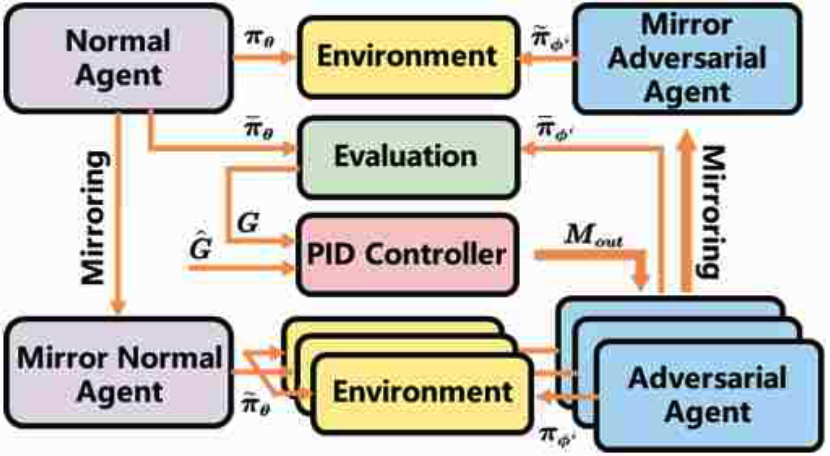
\includegraphics[height=4cm]{lib/graphics/RAEARL Framework.png}
    \caption[Aufbau des RAEARL Frameworks]{Aufbau des RAEARL Frameworks\footnotemark}
    \label{abb:RAEARL}
\end{figure}
\footnotetext{Enthalten in: \cite[][S. 3]{Zhai.2022}}

Abbildung 5 zeigt den getrennten Aufbau des RAEARL Frameworks, in dem die Strategien der originalen Agenten mit $\pi_{\theta}$ bzw. $\pi_{\phi^{i}}$ und jene kopierte Strategien mit $\widetilde{\pi}_{\theta}$ bzw. $\widetilde{\pi}_{\phi^{i}}$ notiert sind. \footcite[Vgl.][S. 3]{Zhai.2022}
Zur Evaluation jeder Epoche und der Bestimmung der kumulierten Belohnung $G$ werden die deterministischen Strategien $\bar{\pi}_{\theta}$ bzw. $\bar{\pi}_{\phi^{i}}$ einbezogen. \footcite[Vgl.][S.3]{Zhai.2022}